\section{Упорядоченные деревья (деревья поиска). Поиск в упорядоченном дереве.  Сбалансированное дерево}
Понятие упорядоченного дерева (бинарного дерева поиска) дано \hyperref[def:bst]{выше}.
\hyperref[sec:tree-ins-del]{Вставка, удаление} и \hyperref[alg:bst-search]{поиск} также были
подвергнуты рассмотрению в разных главах.

Напомним, что дерево называется \textbf{сбалансированным}, если максимум разности высоты любых двух его различных
листьев не превышает единицы.

На сбалансированных деревьев алгоритмы поиска, вставки и удаления не деградируют до $O(n)$
и всегда имеют сложность $O(\log n)$.

Для балансировки деревьев можно использовать несколько подходов.
\subsection{Ручная балансировка}
Самые неэффективный и наивный подход к балансировке. Дерево разворачивается
в линейную отсортированную структуру и собирается заново в уже сбалансированном варианте
(корнем выбирается медиана списка/массива, его детьми --- медианы половин и так далее).
Имеет сложность $O(n^2)$ при использовании списка и $O(n\log n)$ --- массива.

\subsection{Самобалансировка}
Более эффективное способом поддержания сбалансированности дерева является использование
самобалансирующихся структур, в основе которых лежат следующие подходы
\begin{itemize}
  \item Нарушение баланса при добавлении (удалении) узла возникают только на пути от корня к данному узлу,
  не затрагивая остальные поддеревья;
  \item Перенос узла внутри дерева осуществляется быстрее, чем его полная размотка и сборка.
\end{itemize}

Распространенными самобалансирующимися деревьями являются красно-черные и АВЛ-деревья,
которые более подробно рассмотрены в следующем вопросе. В среднем сбалансированным
является \href{https://en.wikipedia.org/wiki/Splay_tree}{Splay-дерево}, которое перестраивает
себя при доступе к данным.

\section{Методы балансировки (самобаоансировки) деревьев}
\subsection{Повороты}
\label{sec:rotations}
Как в красно-черных, так и в АВЛ-деревьях для восстановления баланса используются
\textbf{повороты} --- специальные преобразования структуры дерева.

Разделяют четыре вида поворотов, которые получаются в результате декартова произведения двух признаков:
большие и малые, левые и правые повороты. Правые повороты проводятся симметрично левым, поэтому рассмотрим
только левые.

% TODO: check left and right
В левом малом повороте (рис.~\ref{fig:small-rotation}) корень ($a$) и его правый потомок ($b$)
меняются местами, а левое поддерево ($Q$) нового корня $b$ становится правым потомком старого корня $a$.

В правом малом повороте (рис.~\ref{fig:small-rotation}) корень ($a$) и его левый потомок ($b$)
меняются местами, а правое поддерево ($Q$) нового корня $b$ становится левым потомком старого корня $a$.

Большие повороты являются комбинациями малых. Для левого поворота сперва осуществляется правый поворот
правого ребенка корная, а затем --- левый поворот самого корня (см. рис. \ref{fig:big-rotation}).

\begin{figure}
  \begin{center}
  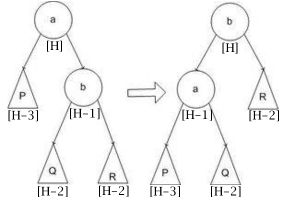
\includegraphics{27-34/small-rotation.jpg}
  \caption{Малый левый поворот}
  \label{fig:small-rotation}
  \end{center}
\end{figure}
\begin{figure}
  \begin{center}
  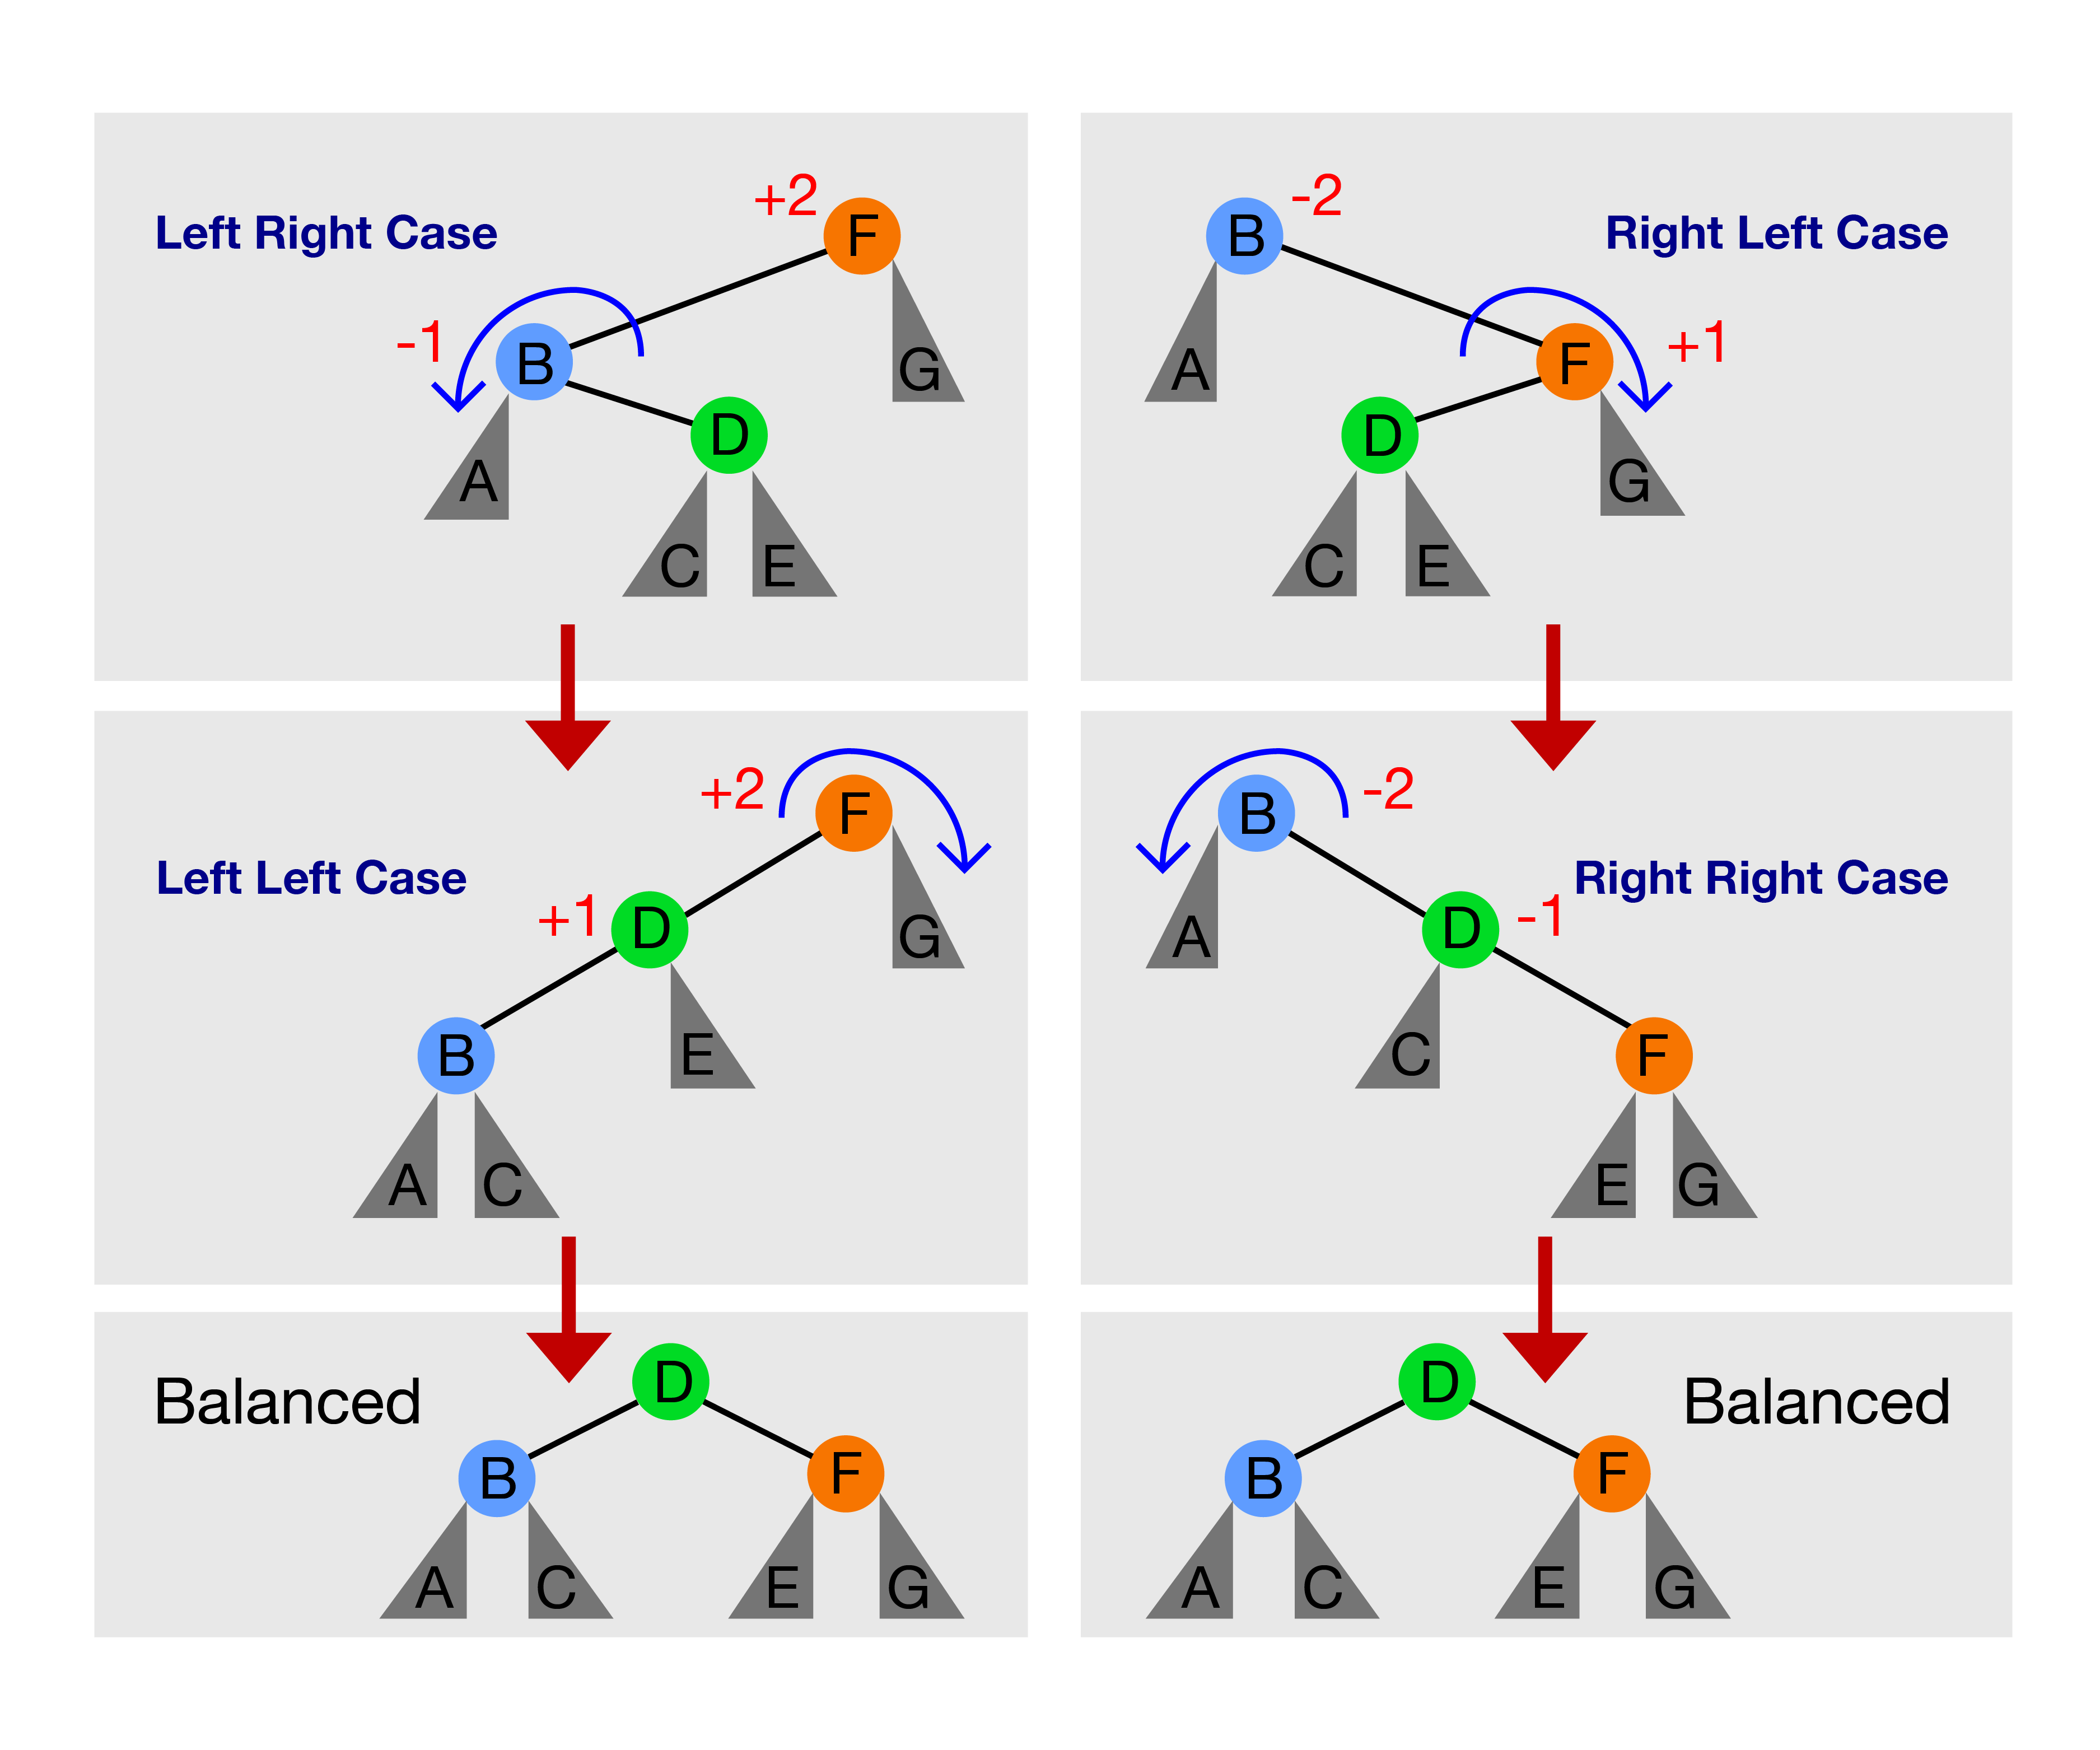
\includegraphics[scale=0.14]{27-34/both-big-rotations.png}
  \caption{Большие \textit{правый} и \textit{левый} повороты (именно в таком порядке!)}
  \label{fig:big-rotation}
  \end{center}
\end{figure}

\subsection{Красно-черное дерево}
В красно-черном дереве (КЧД) для узлов вводится дополнительная характеристика --- цвет.
Правильно построенное КЧД поддерживает следующие инварианты:
\begin{enumerate}
  \item Терминальные узлы фиктивные и не содержат данных;
  \item Корневой и терминальные узлы черные;
  \item У красного узла оба ребенка черные;
  \item Каждый путь от заданного узла до его листового потомка содержит одинаковое количество черных узлов.
\end{enumerate}

Общий алгоритм добавления узла в КЧД таков:
\begin{algorithmic}
  \Procedure{AddNode}{RBTree $t$, Value $v$}
    \State Find a leaf node $u$ to substitute with a new node
    \State $u$ \asgn new Node($v$)
    \State Set $u$'s children to BLACK NIL nodes
    \State $u$.color \asgn RED
    \If{invariant is broken}
      \State $u$.color \asgn BLACK
      \State Fix invariant via rotations
    \EndIf
  \EndProcedure
\end{algorithmic}
\subsection{АВЛ-дерево}
Для каждого узла АВЛ-дерева определяется \textbf{показатель баланса} --- разность
высоты левого и правого поддеревьев данного узла.

Дерево считается сбалансированным, если в каждой его вершине показатель баланса
по модулю не превосходит единицы. АВЛ-деревья сбалансированы не идеально, но близко
к тому и гораздо лучше, чем КЧД.

При удалении или вставке нового узла происходит пересчет балансов у всех вершин дерева на пути к корню
и его восстановление с помощью поворотов.

\subsection{Саморегулирующееся дерево}
Примером саморегулирующихся деревьев является Splay-дерево, которое поддерживает баланс в среднем.
Амортизированная сложность операций поиска, вставки и удаления равна $O(\log n)$. Дерево не хранит
в своих вершинах каких-либо дополнительных данных. При доступе к вершине дерева она продвигается в корень.


\section{Поиск в линейных коллекциях (массивах, списках): линейный, дихотомический, поиск скачками, интерполяционный}
\section{Поиск в многомерных массивах}
\section{Нечеткий поиск - поиск подобной подстроки}
Задача нечеткого поиска (fuzzy string search)~--- найти в тексте или словаре (\textit{haystack}) все подстроки, совпадающие
(начинающиеся) с данной (\textit{needle}) с учетом не более \(k\) ошибок.
Эти алгоритмы являются основными в системах коррекции наборных ошибок
(например \href{https://en.wikipedia.org/wiki/Code_completion}{автодополнение кода} в IDE или подсказки в поисковой строке браузера).
В зависимости от преследуемых целей, существуют и используются различные алгоритмы решения данной задачи в различных постановках.

\subsubsection{Метрики Левенштейна и Хэмминга}
Расстояние Левенштейна~--- минимальное количество односимвольных операций (а именно вставки, удаления, замены),
необходимых для превращения одной последовательности символов в другую.
% cSpell: disable-next-line
Например, расстояние Левенштейна слов \(L(Hello, Hilo) = 2\) (замена `\(e\)' \(\gets\) `\(i\)', вставка `\(l\)').

Расстояние Хэмминга~--- число позиций, в которых соответствующие символы двух слов одинаковой длины различны. Например,
% cSpell: disable-next-line
\(H(Hello, Hillo) = 1\) (замена `\(e\)' \(\gets\) `\(i\)').

Расстояния Хэмминга и Левенштейна, во-первых, являются метриками в математическом смысле слова, во-вторых, позволяют строго
формализовать задачу нечеткого поиска.

Расстояние Левенштейна можно вычислить на основе рекуррентной формулы \[L(a,b) = \begin{cases}
    |a|                                  & \text{если}~|b| = 0,                         \\
    |b|                                  & \text{если}~|a| = 0,                         \\
    L(\text{tail}(a), \text{tail}(b))    & \text{если}~\text{head}(a) = \text{head}(b), \\
    1 + \min \begin{cases}
               L(\text{tail}(a), b)              \\
               L(a, \text{tail}(b))              \\
               L(\text{tail}(a), \text{tail}(b)) \\
             \end{cases} & \text{иначе}                                          \\
  \end{cases}
\]

где \(\text{tail}(\overline{x_1x_2x_3\dots}) = \overline{x_2x_3\dots}\), а \(\text{head}(\overline{x_1x_2x_3\dots}) = x_1\).
Используя также мемоизацию на матрице, можно вычислить расстояние Левенштейна между любыми двумя строками длины \(n\) и \(m\) за
\(O(n\cdot m)\)~--- алгоритм \href{https://neerc.ifmo.ru/wiki/index.php?title=%D0%97%D0%B0%D0%B4%D0%B0%D1%87%D0%B0_%D0%BE_%D1%80%D0%B5%D0%B4%D0%B0%D0%BA%D1%86%D0%B8%D0%BE%D0%BD%D0%BD%D0%BE%D0%BC_%D1%80%D0%B0%D1%81%D1%81%D1%82%D0%BE%D1%8F%D0%BD%D0%B8%D0%B8,_%D0%B0%D0%BB%D0%B3%D0%BE%D1%80%D0%B8%D1%82%D0%BC_%D0%92%D0%B0%D0%B3%D0%BD%D0%B5%D1%80%D0%B0-%D0%A4%D0%B8%D1%88%D0%B5%D1%80%D0%B0}{Вагнера-Фишера}.

\subsubsection{Алгоритм bitap}
Алгоритм \href{https://en.wikipedia.org/wiki/Bitap_algorithm}{bitap} позволяет эффективно с точки зрения реального времени работы процессора вычислять расстояние Хэмминга и
(с модификациями) Левенштейна. При асимптотике \(O(k\cdot n)\), он работает ощутимо быстрее наивного вычисления метрики
Левенштейна для сравнения двух строк, поскольку сравнивает по 32/64 символа за раз. Фактически, это эффективное
распараллеливание наивного линейного алгоритма.

\subsubsection{Алгоритм расширенной выборки}
\begin{center}
  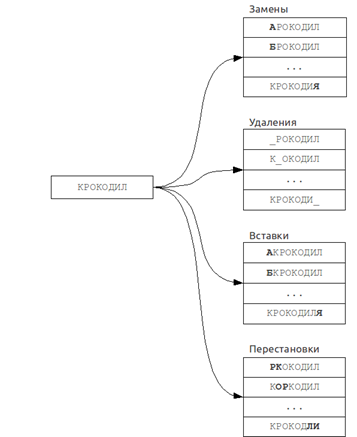
\includegraphics[width=0.3\textwidth]{resources/19-26/inflate.png}
\end{center}
Сводит задачу нечеткого поиска к задаче точного поиска последовательным перебором всех ошибочных трансформаций входной строки.
Неэффективен на больших алфавитах и при больших \(k\), даже при бинарном поиске по словарю временная сложность
\(O((m\cdot |\Sigma|)^k\cdot m\cdot \log{n})\), где \(|\Sigma|\)~--- размер алфавита.

\subsubsection{Метод \(N\)-грамм}
\begin{center}
  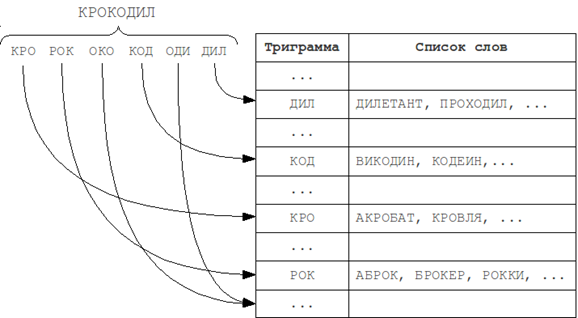
\includegraphics[width=0.3\textwidth]{resources/19-26/n-gramms.png}
\end{center}

Основан на разбиении всех слов в словаре и исходного на \(N\)-граммы~--- последовательности длины \(N\) (обычно \(N = 3\)).
\(N\)-граммы используются для группировки слов в корзины, по которым в дальнейшем и производится поиск.

\subsubsection{\href{https://cs.msu.ru/sites/cmc/files/docs/boycov.pdf}{Хеширование по сигнатуре}, \href{https://en.wikipedia.org/wiki/Locality-sensitive_hashing\#Bit_sampling_for_Hamming_distance}{Locality-sensitive hashing}}

\begin{center}
  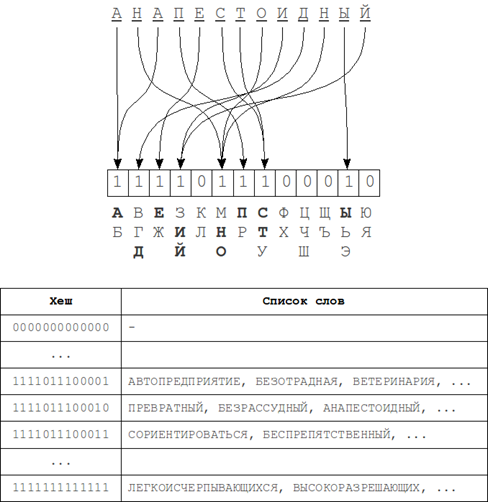
\includegraphics[width=0.3\textwidth]{resources/19-26/hash.png}
\end{center}
Предполагают сопоставление каждому слову специального хеша так, что схожие слова имеют схожие хеш-функции. Тогда поиск следует вести с
теми словами в словаре, у которых близкий или одинаковый хеш с исходной строкой.


\section{Методы сортировки (для линейных коллекций): сортировка вставкой (включением), выбором (выделением), обменом}
\textbf{Сортировка}~--- процесс упорядочивания данных в соответствии с заданным критерием.

Сортировка является фундаментальной операцией при работе с данными, поскольку позволяет работать с ними более
эффективно. В частности, если данные отсортированы, становятся возможным использовать эффективные алгоритмы поиска.

\subsection{Радикальные подходы}
Сортировку можно выполнить аппаратно если число элементов данных невелико~--- строится схема-сортировщик из ячеек памяти
со связями <<каждый с каждым>>, после чего одного прохода достаточно для упорядочивания данных. Очень
неэффективно на больших объемах данных, но очень удобно (и быстро), на малых (например, несколько чисел).

Другая крайность представляет собой перегон элементов в естественно упорядоченную структуру данных~--- двоичное дерево поиска.
После производится обход дерева с извлечением элементов в отсортированном порядке.
Асимптотическая сложность таких алгоритмов даже может быть очень неплохой\footnote{
  Одна из таких сортировок~--- \href{https://en.wikipedia.org/wiki/Splaysort}{splaysort}, использует особое
  сбалансированное дерево поиска~--- \href{https://en.wikipedia.org/wiki/Splay_tree}{splay-дерево}. Такое дерево постоянно перестраивает
  само себя, адаптируясь ко входным данным, работая фактически как кеш. Можно показать, что splaysort работает в среднем не хуже
  \(O(n\log{n})\), а если данные уже частично упорядоченны~--- то даже еще лучше.
}, но основным и серьезным недостатком является
необходимость в \(O(n)\) дополнительной памяти на хранение дерева, при том что данные в дереве дублируют исходные.

% Теперь прейдем к классическим алгоритмам сортировки и их классификации.
% \subsection{Классификация алгоритмов сортировки}
% Алгоритмы сортировки делятся на группы по различным критериям:
% \begin{enumerate}
%   \item По методике сортировки \begin{itemize}
%           \item Внешние~--- сортируют данные на внешних носителях (пример: сортировка слиянием на внешних устройствах).
%           \item Внутренние~--- сортирую данные в оперативной памяти.
%         \end{itemize}
%   \item По способу реализации
%         \begin{itemize}
%           \item Сортировка обменом~--- выявление пар элементов, нарушающих порядок сортировки, и обмен местами.
%                 В обычных последовательных реализациях подход неэффективен, но могут быть хорошо приспособлены для
%                 параллельной реализации.\\
%                 \textbf{Примеры}: <<пузырьковая>> сортировка, \href{https://en.wikipedia.org/wiki/Bitonic_sorter}{битонная} (параллельная) сортировка.
%           \item Сортировка выбором~--- последовательный поиск и отделение от остальных элементов в порядке сортировки.\\
%                 \textbf{Примеры}: \href{https://en.wikipedia.org/wiki/Selection_sort}{сортировка выбором}.
%           \item Сортировка вставками~--- последовательный просмотр элементов (из числа еще неупорядоченных) и вставка их
%                 на соответствующее им место среды уже упорядоченных.\\
%                 \textbf{Примеры}: сортировка вставками, \href{https://en.wikipedia.org/wiki/Shellsort}{сортировка Шелла}.
%         \end{itemize}
%   \item По стабильности \begin{itemize}
%           \item Стабильные~--- гарантируют относительный порядок равных элементов (пример: сортировка вставками).
%           \item Нестабильные~--- в противном случае (пример: быстрая сортировка).
%         \end{itemize}
%   \item По использованию дополнительной памяти \begin{itemize}
%           \item In-place~--- дополнительная память не требуется (пример: пирамидальная сортировка).
%           \item Out-of-place~--- в противном случае (пример: сортировка слиянием).
%         \end{itemize}
%   \item По адаптивности \begin{itemize}
%           \item Адаптивные~--- работают быстрее с частично отсортированными данными (пример: сортировка вставками, \href{https://en.wikipedia.org/wiki/Timsort}{timsort}).
%           \item Неадаптивные~--- выполняют одинаковое количество операций вне зависимости от упорядоченности входных данных
%                 (пример: пирамидальная сортировка).
%         \end{itemize}
% \end{enumerate}

Приведем основные (простейшие) алгоритмы сортировки: сортировку <<пузырьком>>, вставками и выбором.

\subsection{Обменные сортировки. Сортировка <<пузырьком>>}
Обменные сортировки основаны на принципе выявления пар элементов, нарушающих порядок сортировки, и обмену их местами.
В обычных последовательных реализациях подход неэффективен, но могут быть хорошо приспособлены для параллельной реализации.

Примеры:
\begin{itemize}
  \item <<пузырьковая>> сортировка;
  \item \href{https://en.wikipedia.org/wiki/Bitonic_sorter}{битонная} (параллельная) сортировка.
\end{itemize}

<<Пузырьковая>> сортировка является простейшим алгоритмом сортировки и имеет временную сложность \(O(n^2)\), где \(n\)~--- число элементов коллекции.
Эта сортировка не требует дополнительной памяти и произвольного доступа в коллекцию (в частности, её можно применить для сортировки связных
списков), однако высокая асимптотика и низкая скорость делают ее пригодной разве что для обучения курсу ОАиП.

\begin{minted}{cpp}
void BubbleSort(int *array, size_t size) {
  bool swapped;
  for (int i = 0; i < n - 1; i++) {
    swapped = false;
    for (int j = 0; j < n - i - 1; j++) {
      if (arr[j] > arr[j + 1]) {
        std::swap(arr[j], arr[j + 1]);
        swapped = true;
      }
    }
    
    if (!swapped) {
      break;
    }
  }
}
\end{minted}

\subsection{Сортировка вставками}

Сортировки вставками осуществляют последовательный просмотр элементов (из числа еще неупорядоченных) и вставка их на соответствующее
им место среды уже упорядоченных.

Приведем примеры:
\begin{itemize}
  \item сортировка вставками;
  \item \href{https://en.wikipedia.org/wiki/Shellsort}{сортировка Шелла}.
\end{itemize}

Insertion sort~--- классическая сортировка вставками. Данный алгоритм условно разделяет массив на два подмассива, их которых первый отсортирован,
а второй еще нет. Последовательно убирая элементы второго подмассива и вставляя их в уже отсортированный первый, массив оказывается
отсортирован за \(O(n^2)\) в худшем случае. Однако insertion sort~--- крайне эффективный с точки зрения машинного времени алгоритм; на небольших
объемах данных, которые зачастую также уже частично упорядоченны, данная сортировка превосходит большинство других алгоритмов.

\begin{minted}{cpp}
void InsertionSort(int *array, size_t n) {
  size_t i = 1;
  while (i < n) {
    size_t j = i;
    while (j > 0 && array[j - 1] > array+[j]) {
      std::swap(array[j], array[j - 1]);
      --j;
    }
    ++i;
  }
}
\end{minted}

Сортировка <<пузырьком>> и сортировка вставками очень похожи; можно даже показать, что их сортировочные
сети \href{https://ru.wikipedia.org/wiki/Сеть_сортировки}{совпадают при разрешении параллельных вычислений}.

\subsection{Сортировка выбором}
Сортировка выбором предполагает последовательный поиск и отделение от остальных элементов в порядке сортировки.
Данный алгоритм условно разделяет массив на два подмассива, их которых первый отсортирован,
а второй еще нет. После чего из второго подмассива последовательно извлекается наименьший элемент и помещается в конец первой части
пока весь массив не буде отсортирован. Временная сложность составляет \(O(n^2)\) в среднем и худшем случае.

Приведем код данного алгоритма:
\begin{minted}{cpp}
void SelectionSort(int *array, size_t n) {
  for (size_t i = 0; i < n - 1; ++i) {
    size_t j_min = i;
    for (size_t j = i + 1; j < n; ++j) {
      if (array[j] < array[j_min]) {
        j_min = j;
      }
    }

    if (j_min != i) {
      std::swap(array[i], array[j_min]);
    }
  }
}  
\end{minted}

\section{Методы сортировки (для линейных коллекций): сортировка слиянием, "быстрая" сортировка Хоара (quicksort)}
\subsection{QuickSort (быстрая сортировка)}
Time Complexity --- $O(n\log n)$ в среднем, $O(n^2)$
в худшем (если входной массив отсортирован в обратном порядке) случае.
Space Complexity зависит от функции разбиения (функция Хоара дает $\log n$ на стек рекурсивных вызовов).

Быстрая сортировка функционирует по принципу <<разделяй и властвуй>>.
Пусть требуется отсортировать массив из $n$ элементов $a[1\dots n]$ (обе границы включены).
На первом шаге полагаем $l=1$ и $r=n$. Далее придерживаемся следующего алгоритма:
\begin{enumerate}
  \item Вычислить индекс $q$ опорного элемента.
  \item Массив $a[l\dots r]$
  разбивается на два подмассива $a[l\dots q]$ и $a[q+1\dots r]$, таких что каждый элемент $a[l\dots q]$
  меньше или равен $a[q]$, который в свою очередь, не превышает любой элемент подмассива $a[q+1\dots r]$, то есть
  \begin{align*}
    \forall\, n <&q \quad a[n] \leq a[q] \\
    \forall\, m >&q \quad a[q] \leq a[m].
  \end{align*}
  Отметим, что на этом шаге при необходимости некоторые элементы массива переставляются местами так,
  чтобы обеспечить выполнение вышеозначенного свойства.
  \item Подмассивы $a[l\dots q]$ и $a[q+1\dots r]$ сортируются рекурсивно.
\end{enumerate}

Распространенной является функция разбиения Хоара. После выбора опорного элемента $v$
заводятся два индекса: один ($i$) пробегает массив слева направо, а другой ($j$)~--- справа налево.
Когда становится верным $a[i] \geq v \geq a[j]$, элементы $a[i]$ и $a[j]$
меняются местами. После этого просмотр массива продолжается с прежних позиций. Когда индексы,
пересекутся, алгоритм завершается.

Отметим, что в качестве опорного можно выбирать абсолютно любой элемент массива
(даже всегда первый, но при такой реализации сложность любого случая будет $\Theta(n^2)$).

Если кому-либо известен алгоритм функции разбиения, то он может злонамеренно соорудить
такой массив, на котором функция быстрой сортировки уйдет в $O(n^2)$ и/или возникнет
переполнение стека. Чтобы избежать этого, в качестве опорного можно выбирать случайный
элемент массива.

Ниже приведен алгоритм Quicksort с разбиением Хоара.
\begin{minted}{C++}
/// a - массив, который сортируется
/// l - левая граница сортируемого отрезка
/// r - правая граница
int Partition(int *a, int l, int r) {
  int v = a[l + (r - l) / 2];
  int i = l;
  int j = r;
  while (i <= j) {
    while (a[i] < v) {
      ++i;
    }
    while (a[j] > v) {
      --j;
    }
    if (i >= j) {
      break;
    }
    std::swap(a[i++], a[j--]);
  }
  return j;
}

void Quicksort(int *a, int l, int r) {
  if (l < r) {
    int q = Partition(a, l, r);
    Quicksort(a, l, q);
    Quicksort(a, q + 1, r);
  }
}
\end{minted}

\subsection{Сортировка слиянием}
Данный алгоритм также использует стратегию <<разделяй и властвуй>>, рекурсивно сортируя
поданный на вход массив следующим образом:
\begin{enumerate}
  \item Массив разделяется на два подмассива так, чтобы их длины отличались не больше,
        чем на единицу;
  \item Каждый из подмассивов сортируется по отдельности рекурсивным вызовом;
  \item Посортированные массивы объединяются в один. Первый элемент результирующего 
        массива равен наименьшему из элементов подмассивов и так далее.
\end{enumerate}

Нетрудно заметить, что такая реализация потребует $O(n)$ дополнительной памяти.
Существует реализация сортировки слиянием, которая не требует дополнительной памяти,
однако она имеет большую временную сложность: $O(\log^2 n)$ против $O(\log n)$.
Ниже приведена реализация обычного алгоритма сортировки слиянием. Здесь используются
два массива, которые поочередно меняются местами. В каждом из этих массивов
в данный момент времени сортируется только одна половина исходного массива.

\begin{minted}{C++}
int *MergesortImpl(int *up, int *down, int left, int right) {
  if (left == right) {
    down[left] = up[left];
    return down;
  }

  unsigned int middle = left + (right - left) / 2;

  int *l_buff = MergesortImpl(up, down, left, middle);
  int *r_buff = MergesortImpl(up, down, middle + 1, right);

  int *target = l_buff == up ? down : up;

  unsigned int l_cur = left, r_cur = middle + 1;
  for (unsigned int i = left; i <= right; i++) {
    if (l_cur <= middle && r_cur <= right) {
      if (l_buff[l_cur] < r_buff[r_cur]) {
        target[i] = l_buff[l_cur];
        l_cur++;
      } else {
        target[i] = r_buff[r_cur];
        r_cur++;
      }
    } else if (l_cur <= middle) {
      target[i] = l_buff[l_cur];
      l_cur++;
    } else {
      target[i] = r_buff[r_cur];
      r_cur++;
    }
  }
  return target;
}

void Mergesort(int *array, int len) {
  int *back = new int[len];
  std::copy(array, array + len, back);
  int *sorted = MergesortImpl(array, back, 0, len - 1);
  if (sorted != array) {
    std::copy(back, back + len, array);
  }
  delete[] back;
}
\end{minted}